\documentclass[spanish, c]{beamer}

\usepackage[utf8]{inputenc}
%\usepackage[spanish, mexico]{babel}
\usepackage{amsmath}
\usepackage{mathtools}
\usepackage{hyperref}
\usepackage{xcolor}
\usepackage{color}
\usepackage{ragged2e}
\usepackage{mathrsfs}
\usepackage{csquotes}
\usepackage{listings}
\usepackage[scaled]{beramono}
\usepackage[T1]{fontenc}
\usepackage{matlab-prettifier}
\usepackage{graphicx}
\usepackage{booktabs}
\usepackage{gensymb}

\renewcommand{\indent}{\hspace*{2em}}

% \usepackage{tikz}

% \usetikzlibrary{fit, shapes, arrows}

% \usepackage{courier}
% \usepackage{subfigure}
% \usepackage{enumerate}
% \usepackage{algorithmic}
% \usepackage{algorithm}

% \usepackage{listings}
% \usepackage{lstlinebgrd}

\usetheme{Boadilla}
\usefonttheme[onlymath]{serif}

\newcommand{\matlab}[1]{\lstinline[style=Matlab-editor]!#1!}
\newcommand\blfootnote[1]{%
\begingroup
\renewcommand\thefootnote{}\footnote{#1}%
\addtocounter{footnote}{-1}%
\endgroup
}

\lstset
{
    language = Matlab,
    style = Matlab-editor,
    basicstyle = \mlttfamily\scriptsize,
    escapechar = `,
    numbers = left,
    frame = tb,
}

\lstdefinestyle{output}
{
    language = {},
    basicstyle = \mlttfamily\scriptsize,
    escapechar = `,
    numbers = none,
    showtabs = false,
   	showstringspaces = false,
}

\makeatletter
\renewcommand*\env@matrix[1][*\c@MaxMatrixCols c]{%
  \hskip -\arraycolsep
  \let\@ifnextchar\new@ifnextchar
  \array{#1}}
\makeatother

% Sets the templates
\definecolor{navyblue}{RGB}{0, 0, 128}
\definecolor{crimson}{RGB}{128, 16, 0}

\setbeamertemplate{navigation symbols}{}
\setbeamertemplate{headline}{}
\setbeamertemplate{title page}[default][colsep=-4bp,rounded=true]
\setbeamertemplate{footline}[frame number]
\setbeamertemplate{bibliography item}[text]
\setbeamertemplate{theorems}[numbered]

\setbeamercolor{title}{fg=navyblue, bg=white}
\setbeamercolor{frametitle}{fg=navyblue, bg=white}
\setbeamercolor{structure}{fg=navyblue}
\setbeamercolor{button}{fg=white,bg=navyblue}

\setbeamercovered{transparent}

\title{Álgebra Matricial, Determinantes y Regla de Sarrus}
\subtitle{Aplicación de Métodos Numéricos al Ambiente Construido \\ (CV1012)}
\author{
    \texorpdfstring{
        \begin{center}
            M.C. Xavier Sánchez Díaz \\
            \href{mailto:sax@tec.mx}{\texttt{sax@tec.mx}}
        \end{center}
    }
    {M.C. Xavier Sánchez Díaz}
}

\institute[Tecnológico de Monterrey]{
\includegraphics[scale=0.5]{../img/logo}}
\date{}

\begin{document}

\setlength{\rightskip}{0pt}

\begin{frame}[plain]
    \titlepage        
\end{frame}

\begin{frame}{Outline}
    \tableofcontents
\end{frame}

\section{Álgebra Matricial y Ecuaciones}

\begin{frame}{Esfuerzos en una armadura}{Álgebra Matricial y Ecuaciones}
    Queremos encontrar las fuerzas y reacciones asociadas a una armadura estáticamente determinada:
    \begin{center}
        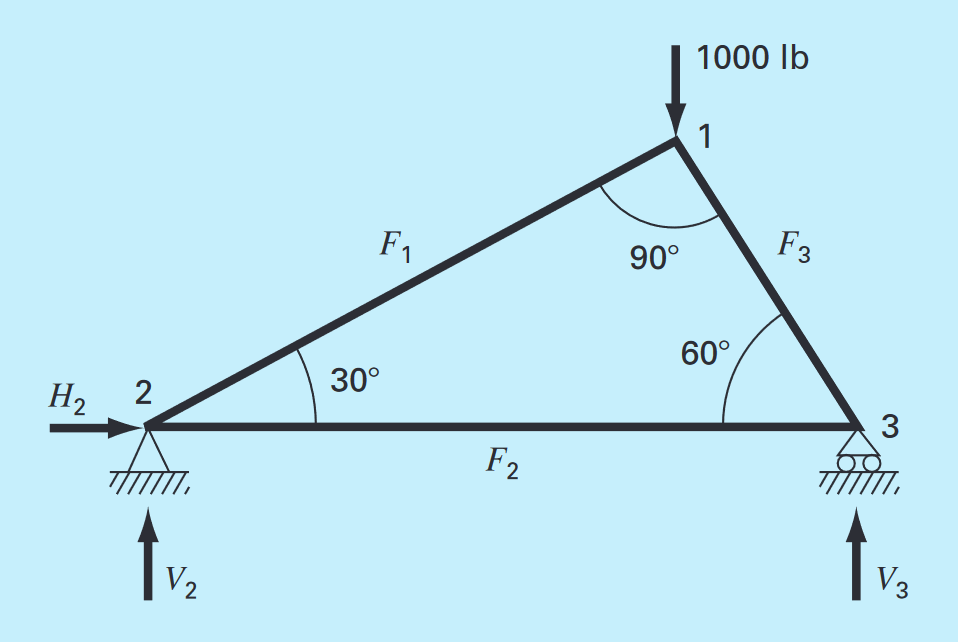
\includegraphics[width=0.57\textwidth]{truss01.png}
    \end{center}    
    con fuerzas ($F_i$) de tensión o compresión en cada nodo, y reacciones externas ($H_2, V_2, V_3$) que son las fuerzas de interacción de la armadura con la superficie en la que se encuentra.
\end{frame}

\begin{frame}{Esfuerzos en una armadura}{Álgebra Matricial y Ecuaciones}
    Cuyo sistema de cuerpo libre es el siguiente\blfootnote{Imágenes tomadas de Chapra \& Canale - Numerical Methods for Engineering}:
    \begin{center}
        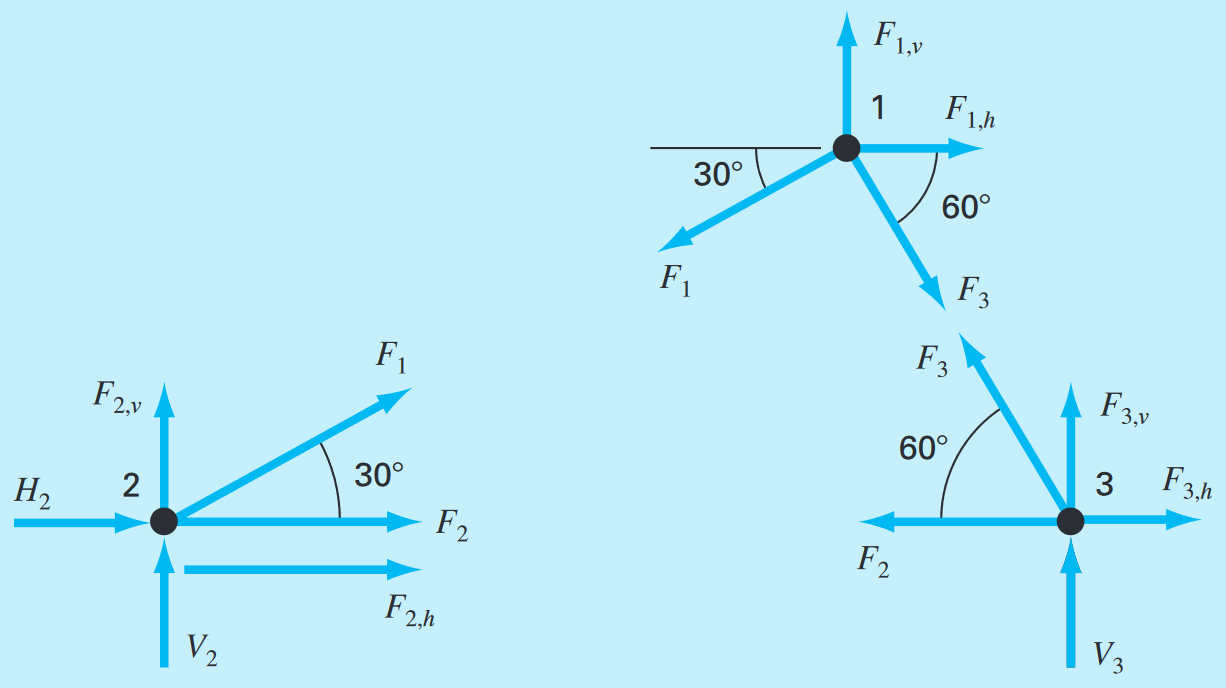
\includegraphics[width=0.9\textwidth]{truss02.png}
    \end{center}
\end{frame}

\begin{frame}{Generando ecuaciones}{Álgebra Matricial y Ecuaciones}
    Podemos generar ecuaciones viendo el diagrama, sabiendo que la suma de fuerzas en cada nodo debe ser de 0:
    \bigskip
    Nodo 1:
    \begin{itemize}
        \item $\sum F_H = 0 = -F_1 \cos 30\degree + F_3 \cos 60\degree + F_{1,h}$
        \item $\sum F_V = 0 = -F_1 \sin 30\degree - F_3 \sin 60\degree + F_{1,v}$
    \end{itemize}
    Nodo 2:
    \begin{itemize}
        \item $\sum F_H = 0 = F_2 + F_1 \cos 30\degree + F_{2, h} + H_2$
        \item $\sum F_V = 0 = F_1 \sin 30\degree + F_{2,v} + F_{2, h} + V_2$
    \end{itemize}
    Nodo 3:
    \begin{itemize}
        \item $\sum F_H = 0 = -F_2 -F_3 \cos 60\degree + F_{3,h}$
        \item $\sum F_V = 0 = F_3 \sin 60\degree + F_{3,v} + V_3$
    \end{itemize}
\end{frame}

\begin{frame}{Acomodando ecuaciones}{Álgebra Matricial y Ecuaciones}
    Siguiendo orden alfabético para las incógnitas ($F_1, F_2, F_3, H_2, V_2, V_3$) y las ecuaciones, entonces tenemos el siguiente sistema de 6 ecuaciones con 6 incógnitas:
    
    $$\begin{bmatrix*}[r]%
        0.866 & 0.0 & -0.5 & 0.0 & 0.0 & 0.0 \\
        0.5 & 0.0 & 0.866 & 0.0 & 0.0 & 0.0 \\
    -0.866 & -1.0 & 0.0 & -1.0 & 0.0 & 0.0 \\
    -0.5 & 0.0 & 0.0 & 0.0 & -1.0 & 0.0 \\
    0.0 & 1.0 & 0.5 & 0.0 & 0.0 & 0.0 \\
    0.0 & 0.0 & -0.866 & 0.0 & 0.0 & -1.0\end{bmatrix*}$$

    \bigskip
    Con un vector de fuerzas resultantes ($F_{1,h}, F_{1,v}, F_{2,h}, F_{2,v}, F_{3,h}, F_{3,v}$) de $$[0, -1000, 0, 0, 0, 0]^T$$
\end{frame}

\begin{frame}{Resolviendo el sistema de ecuaciones}{Álgebra Matricial y Ecuaciones}
    El sistema lo podemos resolver usando \textbf{Eliminación Gaussiana} (aunque sería un poco complicado) o bien usando \alert{factorización LU}\blfootnote{Investiga sobre la factorización LU, es importante que lo conozcas aunque no vayamos a evaluarlo}.

    Tras resolver el sistema, obtenemos el siguiente vector de fuerzas:

    $$ \begin{bmatrix*}[r] -500.0 \\ 433.0127 \\ -866.025 \\ 0.0 \\ 250.0 \\ 750\end{bmatrix*} $$

\end{frame}

\section{Determinantes}

\begin{frame}{Matrices como transformaciones lineales}{Determinantes}

    Ya vimos que las matrices pueden ser usadas para representar datos pero también para representar \textbf{transformaciones}. ¿Qué sucede al realizar esta operación? \pause

    $$\begin{bmatrix*}
        5 & 7 \\ 4 & 3 \\ 6 & 7
    \end{bmatrix*}
    \begin{bmatrix*}
        2 & 0 \\
        0 & 3
    \end{bmatrix*}$$

\end{frame}

\begin{frame}{¿Qué es una determinante?}{Determinantes}
    Se puede obtener un \textbf{escalar} a partir de una matriz \textbf{cuadrada}, al cual llamamos \alert{determinante}.

    El determinante, usualmente denotada como $\det A$, $\det(A)$ o $|A|$, guarda algunas propiedades interesantes con respecto a la matriz de la que se obtuvo: \pause

    \begin{itemize}[<+->]
        \item Si el determinante de una matriz es 0, entonces la matriz es singular (no se puede invertir)
        \item El determinante de una matriz $A$ es igual que el determinante de su transpuesta, $A^T$
        \item El determinante de la matriz inversa $A^{-1}$ de $A$ es igual a $\dfrac{1}{\det A}$
        \item Para dos matrices $A, B$ del mismo tamaño, $\det AB = \det A \times \det B$
        \item Si una matriz tiene una columna o una fila con solamente 0, entonces su determinante es 0
        \item $\det cA = c^n \det A$ para una matriz $A$ de dimensiones $n \times n$
    \end{itemize}
\end{frame}

\begin{frame}{¿Cómo calculo el determinante de una matriz?}{Determinantes}
    Vamos a enfocarnos en solamente dos \textit{tamaños} de matrices. Para lo demás, es conveniente usar software especializado.
    
    Mientras tanto, comencemos para una matriz de 2 $\times$ 2: \pause

\begin{block}{Matrices de 2 $\times$ 2}
    Si $A = \begin{bmatrix*} a & b \\ c & d \end{bmatrix*}$, entonces $\det A = ad - cb$
\end{block} \pause

\begin{exampleblock}{Ejemplo}
    Si $A = \begin{bmatrix}5 & 7 \\ 2 & 3 \end{bmatrix}$,
        entonces su determinante se puede calcular como
        $\det A = (5)(3) - (7)(2) = 15 - 14 = 1$
\end{exampleblock}

\end{frame}

\begin{frame}{Determinantes de matrices de 3 $\times$ 3}{Determinantes}
    Para una matriz de 3 $\times$ 3 es un poco más complicado, pero se puede deducir de manera recursiva:
    $$\det A = \begin{vmatrix*}
        a & b & c \\ d & e & f \\ g & h & i
    \end{vmatrix*} =
     a \begin{vmatrix} \square & \square & \square \\ \square & e & f \\ \square & h & i \end{vmatrix}
    -b \begin{vmatrix} \square & \square & \square \\ d & \square & f \\ g & \square & i \end{vmatrix}
    +c \begin{vmatrix} \square & \square & \square \\ d & e & \square \\ g & h & \square \end{vmatrix}
    $$
    Y como ya sabemos sacar determinantes de matrices de 2 $\times$ 2, entonces llegamos a la fórmula\dots

    \begin{block}{Determinantes de matrices de 3 $\times$ 3}
        $$\det A = aei - ahf - bdi + bgf + cdh - cge$$
    \end{block}
\end{frame}

\section{Regla de Sarrus}

\begin{frame}{La regla de Sarrus}{Determinantes}
    Si agregamos las \alert{primeras dos columnas} a la \textbf{derecha} de la matriz, podemos encontrar un patrón: \pause

    Obtenemos los términos positivos de las \alert{diagonales principales} ($\backslash$):
    $$\begin{bmatrix}
        \color{red} a & \color{blue} b & \color{magenta} c & a & b \\
        d & \color{red} e & \color{blue} f & \color{magenta} d & e \\
        g & h & \color{red} i & \color{blue} g & \color{magenta} h
    \end{bmatrix}$$

    Es decir ${\color{red} aei} + {\color{blue} bfg} + {\color{magenta} cdh}$. Ahora podemos obtener los términos negativos con las \alert{diagonales inversas} (/):
    $$\begin{bmatrix}
        a & b & \color{red} c & \color{blue} a & \color{magenta} b \\
        d & \color{red} e & \color{blue} f & \color{magenta} d & e \\
        \color{red} g & \color{blue} h & \color{magenta} i & g & h
    \end{bmatrix}$$
    
    Es decir ${\color{red} -gec} {\color{blue} -hfa} {\color{magenta} -idb}$.
\end{frame}

% Específicamente, la regla 3 puede verse como $R_i = R_i - \frac{a_{ik}}{a_{jk}}R_j$.

% Los robots
% why is it important
% does it exist in math?
% how to represent it
% how to represent it in matlab
% practical cases

% \section*{Referencias}

% \begin{frame}[t]{Referencias}
    % \nocite{bibID01}
    % \nocite{bibID02}

    % \bibliographystyle{IEEE}
    % \bibliography{biblio}
% \end{frame}

\end{document}